\secspace
\section{Style Mimicry Attacks on Extracted Video Frames}
\label{sec:threat}

Our work considers a previously overlooked variant of the style mimicry
attack, where an attacker extracts individual frames from a video to build
image-based style mimicry models. Next, we introduce the threat model and
consider the limitations of a baseline defense that applies existing
image-based protection tools to individual video frames.

\secspace
\subsection{Threat Model}

\para{Artist/Video creator. } Artists want to share their video 
content online while disallowing unauthorized mimicry using these video frames. 
Artists seeks to protect their video by applying small 
pixel perturbations on the video frames. Following the assumptions made by existing defenses against style mimicry~\cite{shan2023glaze}, we
assume the artists: 
\begin{packed_itemize} 
    \item have access to moderate computing resources (\eg consumer-grade GPUs) commonly used for video rendering; 
    \item add perturbation to video frames before posting videos online; 
    \item have access to some public feature extractor (\eg open-source models such as Stable Diffusion).
\end{packed_itemize}

\para{Attacker. } The attacker's goal is to build a \textit{text-to-image} model
that is able to generate images in the style of the victim artist. We assume the 
attacker 
\begin{packed_itemize} 
\item has access to videos from the victim and leverages frames from
these videos for mimicry; 
\item has significant computational power; 
\item has full access to pretrained, benign text-to-image base models. 
\end{packed_itemize}
Note that our work focuses on text-to-image mimicry, where the attacker's goal
is to {\bf generate images}. We leave text-to-video 
mimicry using video contents to future work. 

\begin{figure}[t]
    \centering
    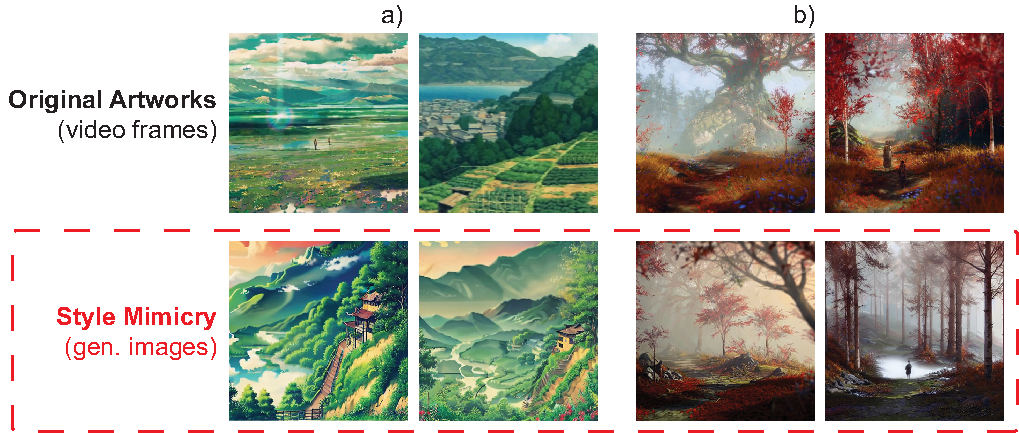
\includegraphics[width=1\columnwidth]{plots/clean-style-mimicry-eps-converted-to.pdf}
    \vspace{-0.2in}
    \caption{Style mimicry on clean video frames successfully mimics style of original video.}
    \label{fig:style-mimicry-baseline}
  \end{figure}
\subsection{Style Mimicry Leveraging Video Frames}

\subsection{A Naive Defense and Its Limitations}
\label{subsec:limitations}

Given the existence of existing tools designed to disrupt art style
mimicry~\cite{shan2023glaze,mist,antidb}, a straightforward solution to
protect video imagery is to simply apply existing protection to each and
every frame of a video.  As discussed in \S\ref{sec:back}, these defenses add
highly-optimized perturbations on each image (a video frame in our case),
misleading the mimicry model to perceive each protected frame as an image with a
completely different style.

Unfortunately, this ``naive'' application of anti-mimicry tools in the video
context has multiple drawbacks, the most critical of which is vulnerability
to a temporal-based adaptive countermeasure.

\para{Vulnerability to countermeasures based on temporal similarity.}  When
applied on individual video frames without coordination, existing protection
methods become vulnerable to advanced countermeasures that exploit
visual similarity across consecutive video frames.

Existing anti-mimicry tools treat each input image independently, with a
randomized component in their generation of perturbation targets for each
image. That means even two runs on the same input image will likely output
two different set of pixel changes. With this in mind, an adaptive mimicry
attack could take several consecutive frames, whose original pixel values are
highly similar, and use them against each other to try to cancel out the
pixel changes made by the protection tools.  An``averaged'' or
``smoothed'' frame generated this way would have much weaker residue
protective perturbations, and would provide a good estimate of the
actual visual feature (i.e. style) carried by the original (unperturbed)
video frames.  An attacker can then use these frames to train a
mimicry model. In \S\ref{sec:eval-limitations}, we provide a detailed study to
validate and quantify this significant vulnerability.


\para{Other limitations: computation and video quality degradation.} The
naive application of protection tools leads to two other challenges. First,
computing independent protection filters on each video frame is
computationally very expensive.  Existing protection tools
(Glaze~\cite{shan2023glaze}, Mist~\cite{mist} and Anti-DB~\cite{antidb}) can
takes up to $\tau=1.5$ minutes to protect a single frame for moderate
GPUs. Protecting a 1 minute video at 30fps (1800 frames) would take 45 hours.
Second, the protective pixel level perturbations are computed independently per
frame and hard to detect on a still image. But when played in a video
sequence, these perturbations cause noticeable flickering effects that
degrade the video quality and viewer experience.
